\section{Gitleaks -- Secret Scanning}
\label{sec:gitleaks}

\subsection{Vấn đề}
Repository YAS chứa nhiều file cấu hình Kubernetes và Docker từ upstream, trong đó có các chuỗi base64-encoded trông giống API keys hoặc secrets. Cần phân biệt giữa \textbf{secrets thật sự mới} (do nhóm vô tình commit) và \textbf{false positives} từ upstream.

\subsection{Công cụ: Gitleaks v8.18.4}
Gitleaks là công cụ mã nguồn mở chuyên quét secrets trong source code. Nhóm sử dụng phiên bản 8.18.4 với chế độ \texttt{--no-git} (quét file trực tiếp, không cần git history).

\subsection{Cấu hình}

\subsubsection{gitleaks.toml}
File cấu hình chính, extend từ bộ rules mặc định và thêm allowlist cho các đường dẫn an toàn:

\begin{lstlisting}[language=bash, caption={gitleaks.toml}]
[extend]
useDefault = true

[allowlist]
paths = [
    '''k8s/.*''',
    '''docker/.*''',
    '''automation-ui/.*''',
    '''.github/.*''',
    '''scripts/.*''',
    '''.*\.md$''',
    '''.*\.json$''',
    '''gitleaks-baseline\.json''',
    '''gitleaks-report\.json'''
]
\end{lstlisting}

\subsubsection{.gitleaksignore}
File chứa danh sách 13 fingerprints cụ thể của các secrets từ upstream cần bỏ qua:

\begin{lstlisting}[caption={.gitleaksignore (trích)}]
# Upstream K8s secrets
6abd7e0e...  # k8s/base secrets
a7f12cb3...  # docker compose credentials
# ... (13 entries)
\end{lstlisting}

\subsubsection{gitleaks-baseline.json}
Baseline trống (\texttt{[]}), đảm bảo chỉ phát hiện secrets \textbf{mới} so với baseline.

\subsection{Luồng quét trong Pipeline}
\begin{enumerate}[noitemsep]
    \item Tải Gitleaks binary (cache nếu đã có)
    \item Kiểm tra baseline file tồn tại
    \item Chạy quét với \texttt{--no-git --config=gitleaks.toml --baseline-path=gitleaks-baseline.json}
    \item Nếu phát hiện secret mới → \textbf{Pipeline FAIL} (\texttt{--exit-code=1})
    \item Nếu không phát hiện → In ``Gitleaks scan PASSED''
\end{enumerate}

\subsection{Kết quả}
\begin{itemize}[noitemsep]
    \item Tất cả các build đều pass Gitleaks scan
    \item 13 false positives từ upstream đã được xử lý qua \texttt{.gitleaksignore}
    \item Console output: \texttt{>>> Gitleaks scan PASSED - no new secrets found}
\end{itemize}

\begin{figure}[H]
    \centering
    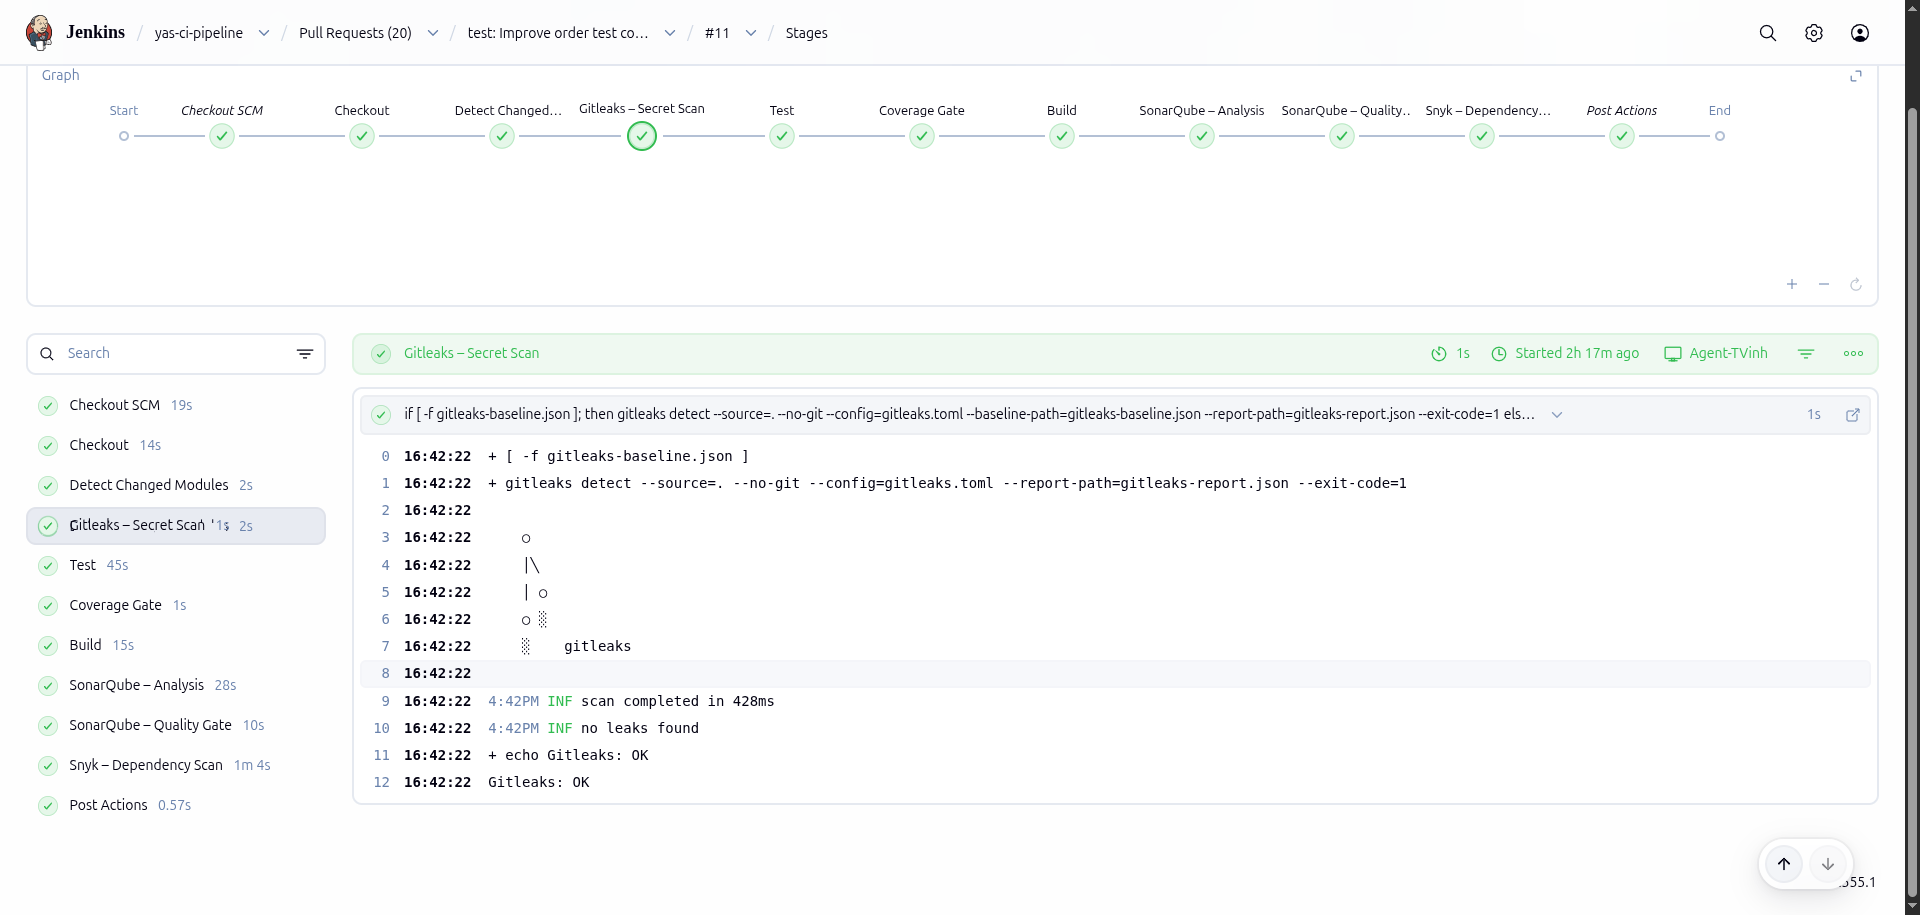
\includegraphics[width=0.9\textwidth]{img/08-jenkins-console-gitleaks-pass.png}
    \caption{Console output hiển thị Gitleaks quét thành công (không phát hiện rò rỉ secret)}
\end{figure}
